\documentclass{article}
\usepackage[margin=2.5cm, top=4cm, headheight=25pt]{geometry}
\usepackage{amsmath, amssymb, enumitem, fancyhdr, graphicx}
\usepackage[indent=20pt]{parskip}
\usepackage[hidelinks]{hyperref}
\usepackage{xcolor}
\usepackage{listings}
\usepackage{subcaption}
\usepackage{url}
\usepackage[most]{tcolorbox}
\usepackage{lastpage}
\usetikzlibrary{arrows, shapes}

\tcbuselibrary{listingsutf8} % Support for lstlistings within tcolorbox

\newtcolorbox[auto counter, number within=section]{question}[1][]{%
    colframe=gray!80,                      % Dark gray frame
    colback=gray!5,                       % Light gray background
    coltitle=black,                        % Black title
    title=\textbf{Question~\thetcbcounter}, % Bold title
    fonttitle=\bfseries\large,             % Subtle title font size
    rounded corners,                   % Slightly more rounded corners
    boxrule=0.25mm,                         % Thinner border for a sleek look
    enhanced,                              % Enhanced box features
    attach boxed title to top left={xshift=2mm, yshift=-2mm},
    boxed title style={colframe=gray!80, colback=gray!5, boxrule=0.25mm},
    % Title styling
    #1
}

\bibliographystyle{IEEEtran}
\graphicspath{{./images/}}

% -- Custom Variables --
\def\me{Rajdeep Gill 7934493}
\def\course{ECE 4260}
\def\labsection{A01}

\def\labno{5}
\def\title{Assignment \labno}

% -- Styling for code snippets --
\lstset{
    basicstyle=\ttfamily\scriptsize,           % Basic font style
    keywordstyle=\color{blue},            % Keywords color
    commentstyle=\color{gray},            % Comments color
    stringstyle=\color{teal},             % Strings color
    numbers=left,                         % Line numbers on the left
    numberstyle=\tiny\color{gray},        % Line number style
    stepnumber=1,                         % Line number step
    numbersep=10pt,                       % Space between line numbers and code
    backgroundcolor=\color{lightgray!10}, % Background color
    frame=single,                         % Adds a frame around the code
    breaklines=true,                      % Line breaking for long lines
    captionpos=b,                         % Caption position
    showspaces=false,                     % Don't show spaces
    showstringspaces=false                % Don't show spaces in strings
}
\renewcommand{\lstlistingname}{Code Snippet}

\renewcommand{\arraystretch}{1.2} % For less-ugly tables
\setlength\parindent{0pt}

%----- Samples 
% Questions:
%   \begin{question}[title=Custom Question Title]
%       Question details
%   \end{question}

% Tables:
%   \begin{table}[htbp]
%       \centering
%       \caption{Table Caption}
%       \begin{tabular}{ll}
%           \toprule
%           \textbf{Column 1} & \textbf{Column 2} \\
%           \midrule
%           Row 1 & Row 2 \\
%           Row 3 & Row 4 \\
%           \bottomrule
%       \end{tabular}
%   \end{table} 

% Figures:
%   Single figure:
%       \begin{figure}[htbp]
%           \centering
%           \includegraphics[width=0.5\textwidth]{example-image}
%           \caption{Figure Caption}
%       \end{figure}
%   Multiple figures:
%       \begin{figure}[htbp]
%           \centering
%           \begin{subfigure}[b]{0.5\textwidth}
%               \includegraphics[width=\textwidth]{example-image-a}
%               \caption{First subfigure}
%           \end{subfigure}
%           \begin{subfigure}[b]{0.5\textwidth}
%               \includegraphics[width=\textwidth]{example-image-b}
%               \caption{Second subfigure}
%           \end{subfigure}
%           \caption{Main figure}
%       \end{figure}

\begin{document}

% --------------------------------------------------------------------------------
% TITLE
% --------------------------------------------------------------------------------

\begin{center}
    \huge \title

    \vspace{2mm}
    \hrule

    \vspace{4mm}
    \large \me

    \vspace{2mm}
    \large \course~\labsection

    \vspace{2mm}
    \today
\end{center}

\vspace{4mm}

% --------------------------------------------------------------------------------
% END TITLE
% --------------------------------------------------------------------------------

\newpage


\vspace{1cm}
\newpage

\pagestyle{fancy}
\fancyhead[L]{\large Assignment \labno}
\fancyhead[R]{\large \me}

\fancyfoot[C]{Page \thepage~of~\pageref{LastPage}}

% --------------------------------------------------------------------------------
% BODY
% --------------------------------------------------------------------------------
\section{Problem 1}

\begin{enumerate}[label=1.\arabic*]
    \item We can find the expectation of $f_U(u)$ as follows:
    \begin{align*}
        \mathbb{E}\left\{e^{-j2\pi f U}\right\}
    \end{align*}

    We have that $g(x) = e^{-j2\pi f x}$ so we use the property:
    \begin{align*}
        \mathbb{E}\left\{g(X)\right\} &= \int_{-\infty}^{\infty} e^{-j2\pi f x} f_U(u) du \\
        &= F_U(f)
    \end{align*}
    \item We know that $f_{Z_{n}}(z_n)$ is the sum of the $n$ independent random variables $X_1, X_2, \ldots, X_n$, thus the PDF will be a convolution of the PDFs of the individual random variables:
    \begin{align*}
        Z_{2} &= X_1 + X_2 \\
        f_{Z_2}(z_2) &= f_{X_1}(x_1) * f_{X_2}(x_2) \\
    \end{align*}
    Now we take the expectation similar to 1.1:
    \begin{align*}
       \mathbb{E}\left\{e^{-j2\pi f Z_2}\right\} &= \int_{-\infty}^{\infty} e^{-j2\pi f z} f_{Z_2}(z) dz \\
       &= F_{Z_2}(f) \\
    \end{align*}

    Now applying the property of the convolution, and the fact they are both indentically distributed:
    \begin{align*}
        F_{Z_2}(f) &= F_{X_1}(f)F_{X_2}(f) \\
        &= F_{X}(f)F_{X}(f) \\
        &= F_{X}(f)^2 \\
    \end{align*}

    \item We can deduce the following:
    \begin{align*}
        F_{Z_n}(f) &= F_{X}(f)^n \\
    \end{align*}

    Using mathematical induction, we can show that this is true for all $n$. First we have our base case, $n = 1$:
    \begin{align*}
        F_{Z_1}(f) &= \mathbb{E}\left\{e^{-j2\pi f Z_1}\right\} = \int_{-\infty}^{\infty} e^{-j2\pi f z} f_{Z_1}(z) dz \\
        &= \int_{-\infty}^{\infty} e^{-j2\pi f z} f_{X}(x) dx \\
        &= F_{X}(f) \\
    \end{align*}
    We also showcased the case for $n=2$ in the previous part. Now we assume that this is true for $n = k$, that is:
    \begin{align*}
        F_{Z_k}(f) &= F_{X}(f)^k \\
    \end{align*}

    Now we show that this is true for $n = k + 1$. We know that we can represent $Z_{k+1}$ as:
    \begin{align*}
        Z_{k+1} = Z_{k} + X_n \\
        f_{Z_{k+1}}(z) &= f_{Z_k}(z) \ast f_{X_n}(x) \\
    \end{align*}
    Taking the expectation of $Z_{k+1}$:
    \begin{align*}
        \mathbb{E}\left\{e^{-j2\pi f Z_{k+1}}\right\} &= \int_{-\infty}^{\infty} e^{-j2\pi f z} f_{Z_{k+1}}(z) dz \\
        &= F_{Z_{k+1}}(f) \\
    \end{align*}

    Using the convolution property:
    \begin{align*}
        F_{Z_{k+1}}(f) &= F_{Z_k}(f)F_{X_n}(f) \\
        &= F_{X}(f)^k F_{X}(f) \\
        &= F_{X}(f)^{k+1} \\
    \end{align*}

    Thus we have shown that this is true for $n = k + 1$. Therefore, by the principle of mathematical induction, we have shown that this is true for all $n \geq 1$.

    \item We know that $S_n$ is defined as the normalized sum of the $n$ independent random variables:
    \begin{align*}
        S_n &= \frac{1}{\sqrt{n}}(X_1 + X_2 + \ldots + X_n) \\
        &= \frac{1}{\sqrt{n}}Z_n
    \end{align*}

    We can now use the property in equation (44):
    \begin{align*}
        \mathbb{E}\left\{e^{-j2\pi f S_n}\right\} &= \mathbb{E}\left\{e^{-j2\pi f \frac{1}{\sqrt{n}}Z_n}\right\} \\
        &= \int_{-\infty}^{\infty} e^{-j2\pi \frac{f}{\sqrt{n}}z} f_{Z_n}(z) dz \\
        &= F_{Z_n}\left(\frac{f}{\sqrt{n}}\right) \\
    \end{align*}

    \item The order-2 Taylor series expansion of the given exponential is:
    \begin{align*}
        e^{-j2\pi \frac{f}{\sqrt{n}}x} &= 1 - j2\pi \frac{f}{\sqrt{n}}x + \frac{1}{2}\left(-j2\pi \frac{f}{\sqrt{n}}x\right)^2 + \ldots \\
        &\approx 1 - \frac{j2\pi f}{\sqrt{n}}x - \frac{2\pi^2 f^2}{n}x^2 \\
    \end{align*}

    \item We can now estimate the fourier transform of $F_X(f/\sqrt{n})$ using (13) and the order-2 Taylor series expansion:
    \begin{align*}
        F_X{f/\sqrt{n}} &= \int_{-\infty}^{\infty} e^{-j2\pi \frac{f}{\sqrt{n}}x} f_X(x) dx \\
        &\approx \int_{-\infty}^{\infty} \left(1 - \frac{j2\pi f}{\sqrt{n}}x - \frac{2\pi^2 f^2}{n}x^2\right) f_X(x) dx \\
        &\approx 1 - \frac{j2\pi f}{\sqrt{n}} \int_{-\infty}^{\infty} x f_X(x) dx - \frac{2\pi^2 f^2}{n} \int_{-\infty}^{\infty} x^2 f_X(x) dx \\
        &\approx 1 - \frac{2\pi^2 f^2}{n} \\
    \end{align*}

    \item We can find the approximation of the Fourier transform of $S_n$ as follows, using (10), (15) and (16):
    \begin{align*}
        F_{S_n}(f) &= \left(F_X\left(\frac{f}{\sqrt{n}}\right)\right)^n \\
        &\approx \left(1 - \frac{2\pi^2 f^2}{n}\right)^n \\
        &\approx e^{-2\pi^2 f^2} \quad \text{as } n \longrightarrow \infty \\
    \end{align*}

    \item Now we can find inverse Fourier transform of $F_{S_n}(f)$. We first recognize that:  
    \begin{align*}
        e^{-\pi x^2} \leftrightarrow e^{-\pi f^2}
    \end{align*}

    In our case, we have a scaled version, so we also apply the scaling property:
    \begin{align*}
        x(at) \leftrightarrow \frac{1}{|a|}X\left(\frac{f}{a}\right)
    \end{align*}

    Rearranging $F_{S_n}(f)$, we can find the scaling factor needed to apply the above property:
    \begin{align*}
        F_{S_n}(f) &\approx e^{-\pi (\sqrt{2\pi}f)^2} \\
    \end{align*}

    Using $a = \sqrt{2\pi}$, we can find the inverse Fourier transform:
    \begin{align*}
        f_{S_n}(t) &\approx \frac{1}{\sqrt{2\pi}} e^{-\pi t^2} \text{as } n \longrightarrow \infty \\
    \end{align*}
\end{enumerate}

\section{Problem 2}
\begin{enumerate}[label=2.\arabic*]
    \item We first show that the length of the two basis vectors is equal to 1:
    \begin{align*}
        \|\Psi_1(t)\| = \left\|\frac{s_1(t)}{\|s_1(t)\|}\right\| = \frac{1}{\|s_1(t)\|}\left\|s_1(t)\right\| = 1 \\
        \|\Psi_2(t)\| = \left\|\frac{d_2(t)}{\|d_2(t)\|}\right\| = \frac{1}{\|d_2(t)\|}\left\|d_2(t)\right\| = 1
    \end{align*}

    We can show that these two vectors are orthogonal to each other:
    \begin{align*}
        \langle \Psi_1(t), \Psi_2(t) \rangle &= \langle \Psi_1(t), \frac{d_2(t)}{\|d_2(t)\|} \rangle \\
        &= \langle \Psi_1(t), \frac{1}{\|d_2(t)\|} (s_2(t) - \alpha_{21}\psi_1(t)) \rangle \\
        &= \frac{1}{\|d_2(t)\|} \left[\alpha_{21} - \alpha_{21}(1)\right] \\
        &= 0
    \end{align*}

    We utilize the fact that $\alpha_{21} = \langle s_2(t), \Psi_1(t) \rangle$ and that the length of $\Psi_1(t) = 1$.

    \item We can express the two signals $s_1(t)$ and $s_2(t)$ in terms of the basis vectors $\Psi_1(t)$ and $\Psi_2(t)$:
    \begin{align*}
        s_1(t) &= \| s_1(t) \| \Psi_1(t) \\
        s_2(t) &= d_2(t) + \alpha_{21} \Psi_1(t) \\
        &= \| d_2(t) \| \Psi_2(t) + \alpha_{21} \Psi_1(t)
    \end{align*}

    We know that from (25) that $\|s_1(t)\| = \sqrt{\mathcal{E}_1}$, then we can write:
    \begin{align*}
        s_1(t) &= \sqrt{\mathcal{E}_1} \Psi_1(t) \\
    \end{align*}

    We can also calculate the length of $d_2(t)$ as follows:
    \begin{align*}
        \langle d_2(t), d_2(t) \rangle &= \int_{-\infty}^{\infty} d_2(t) d_2(t) dt \\
        &= \int_{-\infty}^{\infty} \left(s_2(t) - \alpha_{21}\Psi_1(t)\right)^2 dt \\
        &= \int_{-\infty}^{\infty} s_2(t) s_2(t) dt - 2\alpha_{21} \int_{-\infty}^{\infty} s_2(t) \Psi_1(t) dt + \alpha_{21}^2 \int_{-\infty}^{\infty} \Psi_1(t) \Psi_1(t) dt \\
        &= \mathcal{E}_2 - 2\alpha_{21} \times \alpha_{21} + \alpha_{21}^2 \times 1 \\
        &= \mathcal{E}_2 - \alpha_{21}^2
        \implies \|d_2(t)\| = \sqrt{\mathcal{E}_2 - \alpha_{21}^2}
    \end{align*}

    Now with the results from above, we express these two signals in terms of the basis vectors in their geomtric form:
    \begin{align*}
        s_1(t) = \sqrt{\mathcal{E}_1} \Psi_1(t) &\longleftrightarrow \mathbf{s_1} = \begin{bmatrix}
            \sqrt{\mathcal{E}_1} \\
            0
        \end{bmatrix} \\
        s_2(t) = \sqrt{\mathcal{E}_2 + \alpha_{21}^2} \Psi_2(t) + \alpha_{21} \Psi_1(t) &\longleftrightarrow \mathbf{s_2} = \begin{bmatrix}
            \alpha_{21} \\
            \sqrt{\mathcal{E}_2 - \alpha_{21}^2}
        \end{bmatrix} \\
    \end{align*}



    \item We can show the following identities:
    \begin{enumerate}[label=\alph*.]
        \item $\|s_1(t)\|^2 = \|\mathbf{s_1}\|^2$
        \begin{align*}
            \|s_1(t)\|^2 &= \int_{-\infty}^{\infty} s_1(t) s_1(t) dt \\
            &= \sqrt{\mathcal{E}_1}^2 = \mathcal{E}_1 \\
            \|\mathbf{s_1}\|^2 &= \left\|\begin{bmatrix}
                \sqrt{\mathcal{E}_1} \\
                0
            \end{bmatrix}\right\|^2 = \left(\sqrt{\left(\sqrt{\mathcal{E}_1}\right)^2 + 0^2}\right)^2 = \mathcal{E}_1 \\
            \implies \|s_1(t)\|^2 = \|\mathbf{s_1}\|^2
        \end{align*}

        \item $\|s_2(t)\|^2 = \|\mathbf{s_2}\|^2$
        \begin{align*}
            \|s_2(t)\|^2 &= \int_{-\infty}^{\infty} s_2(t) s_2(t) dt \\
            &= \sqrt{\mathcal{E}_2}^2 = \mathcal{E}_2 \\
            \|\mathbf{s_2}\|^2 &= \left\|\begin{bmatrix}
                \alpha_{21} \\
                \sqrt{\mathcal{E}_2 - \alpha_{21}^2}
            \end{bmatrix}\right\|^2 = \alpha_{21}^2 + \sqrt{\mathcal{E}_2 - \alpha_{21}^2}^2 = \alpha_{21}^2 + \mathcal{E}_2 - \alpha_{21}^2 = \mathcal{E}_2 \\
            \implies \|s_2(t)\|^2 = \|\mathbf{s_2}\|^2
        \end{align*}

        \item $\| s_2(t) - s_1(t)\|^2 = \|\mathbf{s_2} - \mathbf{s_1}\|^2$
        \begin{align*}
            \|s_2(t) - s_1(t)\|^2 &= \int_{-\infty}^{\infty} \left(s_2(t) - s_1(t)\right)^2 dt \\
            &= \int_{-\infty}^{\infty} \left(s_2^2(t) - 2s_2(t)s_1(t) + s_1^2(t)\right)\, dt \\
            &= \mathcal{E}_2 + \mathcal{E}_1 - 2\int_{-\infty}^{\infty} s_2(t)s_1(t) dt \\
            &= \mathcal{E}_2 + \mathcal{E}_1 - 2\int_{-\infty}^{\infty} 
            \big(\alpha_{21} \Psi_1(t) + \sqrt{\mathcal{E}_2 - \alpha_{21}^2}\Psi_2(t)\big)\big(\sqrt{\mathcal{E}_1}\Psi_1(t)\big) \, dt \\
            &= \mathcal{E}_2 + \mathcal{E}_1 - 2\bigg(\alpha_{21}\sqrt{\mathcal{E}_1} 
            \int_{-\infty}^{\infty} \Psi_1(t) \Psi_1(t) dt \notag \\ 
            &\quad + \sqrt{\mathcal{E}_2 - \alpha_{21}^2}\int_{-\infty}^{\infty} \Psi_2(t) \Psi_1(t) dt\bigg) \\
            &= \mathcal{E}_2 + \mathcal{E}_1 - 2\alpha_{21}\sqrt{\mathcal{E}_1} \\
            \|\mathbf{s_2} - \mathbf{s_1}\|^2 &= \left\|
            \begin{bmatrix}
                \alpha_{21} \\
                \sqrt{\mathcal{E}_2 - \alpha_{21}^2}
            \end{bmatrix} - 
            \begin{bmatrix}
                \sqrt{\mathcal{E}_1} \\
                0   
            \end{bmatrix}
            \right\|^2 \\
            &= \left\|
            \begin{bmatrix}
                \alpha_{21} - \sqrt{\mathcal{E}_1} \\
                \sqrt{\mathcal{E}_2 - \alpha_{21}^2}
            \end{bmatrix}
            \right\|^2 \\
            &= (\alpha_{21} - \sqrt{\mathcal{E}_1})^2 + \left(\sqrt{\mathcal{E}_2 - \alpha_{21}^2}\right)^2 \\
            &= \alpha_{21}^2 - 2\alpha_{21}\sqrt{\mathcal{E}_1} + \mathcal{E}_1 + \mathcal{E}_2 - \alpha_{21}^2 \\
            &= \mathcal{E}_1 + \mathcal{E}_2 - 2\alpha_{21}\sqrt{\mathcal{E}_1} \\
            &\implies \|s_2(t) - s_1(t)\|^2 = \|\mathbf{s_2} - \mathbf{s_1}\|^2
        \end{align*}
        
        \item $\langle s_2(t), s_1(t) \rangle = \langle \mathbf{s_2}, \mathbf{s_1} \rangle$

        \begin{align*}
            \langle s_2(t), s_1(t) \rangle &= \int_{-\infty}^{\infty} s_2(t) s_1(t) dt \\
            &= \int_{-\infty}^{\infty} \left(\alpha_{21} \Psi_1(t) + \sqrt{\mathcal{E}_2 - \alpha_{21}^2}\Psi_2(t)\right)\left(\sqrt{\mathcal{E}_1}\Psi_1(t)\right) dt \\
            &= \alpha_{21}\sqrt{\mathcal{E}_1} \int_{-\infty}^{\infty} \Psi_1(t) \Psi_1(t) dt + \sqrt{\mathcal{E}_2 - \alpha_{21}^2}\int_{-\infty}^{\infty} \Psi_2(t) \Psi_1(t) dt \\
            &= \alpha_{21}\sqrt{\mathcal{E}_1} + \sqrt{\mathcal{E}_2 - \alpha_{21}^2} \cdot 0 \\
            &= \alpha_{21}\sqrt{\mathcal{E}_1} \\
            \langle \mathbf{s_2}, \mathbf{s_1} \rangle &= \mathbf{s_2}^T \mathbf{s_1} \\
            &= \begin{bmatrix}
                \alpha_{21} & \sqrt{\mathcal{E}_2 - \alpha_{21}^2}
            \end{bmatrix}
            \begin{bmatrix}
                \sqrt{\mathcal{E}_1} \\
                0
            \end{bmatrix} \\
            &= \alpha_{21}\sqrt{\mathcal{E}_1} + \sqrt{\mathcal{E}_2 - \alpha_{21}^2} \cdot 0 \\
            &= \alpha_{21}\sqrt{\mathcal{E}_1} \\
            &\implies \langle s_2(t), s_1(t) \rangle = \langle \mathbf{s_2}, \mathbf{s_1} \rangle
        \end{align*}
    \end{enumerate}

    \item Given the signal $s_i(t)$, we can find hte energy $\mathcal{E}_i$ for $i = 1, 2$ as follows:
    \begin{align*}
        \mathcal{E}_i &= \int_{-\infty}^{\infty} s_i(t) s_i(t) dt \\
        &= \int_{-\infty}^{\infty} \left(\sqrt{\frac{2\mathcal{E}_b}{T}}\cos\left(2\pi f_i t\right)\right)^2 \, dt \\
        &= \int_{0}^{T} \left(\sqrt{\frac{2\mathcal{E}_b}{T}}\cos\left(2\pi f_i t\right)\right)^2 \, dt \\
        &= \frac{2\mathcal{E}_b}{T} \int_{0}^{T} \cos^2\left(2\pi f_i t\right) dt \\
        &= \frac{2\mathcal{E}_b}{T} \int_{0}^{T} \frac{1+ \cos(4\pi f_i t)}{2} dt \\
        &= \frac{2\mathcal{E}_b}{T} \cdot \frac{1}{2T} \\
        &= \mathcal{E}_b 
    \end{align*}

    We see that the final result is independent of $f_i$, so we have shown that $\mathcal{E}_1 = \mathcal{E}_2 = \mathcal{E}_b$.

    \item We can find the two orthonormal basis vectors $\Psi_1(t)$ and $\Psi_2(t)$ as follows:
    \begin{align*}
        \Psi_1(t) &= \frac{s_1(t)}{\|s_1(t)\|} = \frac{s_1(t)}{\sqrt{\mathcal{E}_b}} = \sqrt{\frac{2}{T}} \cos(2\pi f_1 t) \\
        \Psi_2(t) &= \frac{s_2(t)}{\|s_2(t)\|} = \frac{s_2(t)}{\sqrt{\mathcal{E}_b}} = \sqrt{\frac{2}{T}} \cos(2\pi f_2 t) \\
    \end{align*}

    \item To express $P_e$ in terms of the SNR per bit, we need to find the distance $d_{12}$ between the two signals $s_1(t)$ and $s_2(t)$:
    \begin{align*}
        d_{12}^2 &= \|s_2(t) - s_1(t)\|^2 \\
        &= \int_{-\infty}^{\infty} \left(s_2(t) - s_1(t)\right)^2 dt \\
        &= \sum_{i=1}^{2} (s_{2i} - s_{1i})^2 \\
        &= \left(0 - \sqrt{\mathcal{E}_b}\right)^2 + \left(\sqrt{\mathcal{E}_b} - 0\right)^2 \\
        &= 2\mathcal{E}_b \\
        \implies d_{12} &= \sqrt{2\mathcal{E}_b}
    \end{align*}

    Therefore, our $P_e$ can be expressed as:
    \begin{align*}
        P_e = Q\left(\frac{d_{12}}{\sqrt{2N_0}}\right) = Q\left(\frac{\sqrt{2\mathcal{E}_b}}{\sqrt{2N_0}}\right) = Q\left(\sqrt{\frac{\mathcal{E}_b}{N_0}}\right) = Q \left(\sqrt{\frac{\text{SNR}}{2}}\right)
    \end{align*}
\end{enumerate}


\section{Problem 3}
\begin{enumerate}[label=3.\arabic*]
    \item \begin{enumerate}[label=\alph*.]
        \item We can find the correlation coefficient, $\rho$, as follows:
        \begin{align*}
            \rho &= \frac{1}{\sqrt{\mathcal{E}_1 \mathcal{E}_2}} \int_{-\infty}^{\infty} s_1(t) s_2(t) dt \\
            &= \frac{1}{\sqrt{\mathcal{E}_1 \mathcal{E}_2}} \int_{0}^{T} \left(\sqrt{\frac{2\mathcal{E}_b}{T}}\cos(2\pi \left[f_c + \frac{\Delta f}{2}\right]t)\right)\left(\sqrt{\frac{2\mathcal{E}_b}{T}}\cos(2\pi \left[f_c - \frac{\Delta f}{2}\right] t)\right) dt \\
        \end{align*}
        From problem 2, we know that $\mathcal{E}_1 = \mathcal{E}_2 = \mathcal{E}_b$, so we can simplify this to:
        \begin{align*}
            \rho = \frac{2}{T} \int_{0}^{T} \cos\left(2\pi \left[f_c + \frac{\Delta f}{2}\right]t\right)\cos\left(2\pi \left[f_c - \frac{\Delta f}{2}\right] t\right) dt \\
        \end{align*}
        
        We can use the cosine product identity:
        \begin{align*}
            \cos(a)\cos(b) = \frac{1}{2}\left(\cos(a+b) + \cos(a-b)\right) \\
            a+b = 2\pi \left[ f_c + \frac{\Delta f}{2} \right]t + 2\pi \left[ f_c - \frac{\Delta f}{2} \right]t = 4\pi f_c t\\
            a-b = 2\pi \left[ f_c + \frac{\Delta f}{2} \right]t - 2\pi \left[ f_c - \frac{\Delta f}{2} \right] t = 2\pi \Delta f t
        \end{align*}
        
        We can now substitute this into our equation:
        \begin{align*}
            \rho &= \frac{2}{T}\int_{0}^{T} \frac{1}{2}\left(\cos(4\pi f_c t) + \cos(2\pi \Delta f t)\right) dt \\
            &= \frac{1}{T} \left[\frac{\sin(4\pi f_c t)}{4\pi f_c} + \frac{\sin(2\pi \Delta f t)}{2\pi \Delta f}\right] \Bigg|_{0}^{T} \\
            &= \frac{1}{T} \left[\frac{\sin(4\pi f_c T)}{4\pi f_c} + \frac{\sin(2\pi \Delta f T)}{2\pi \Delta f}\right]
        \end{align*}
        
        Since $f_c \gg 1$, the first term with $4\pi f_c$ in the denominator will be negligible, and thus our approximation is:
        \begin{align*}
            \rho &\approx \frac{1}{T} \cdot \frac{\sin(2\pi \Delta f T)}{2\pi \Delta f} \\
            &\approx \text{sinc}(2\Delta f T) \\
        \end{align*}

        \item The sketch of this is as follows:
        \begin{figure}[ht!]
            \centering
            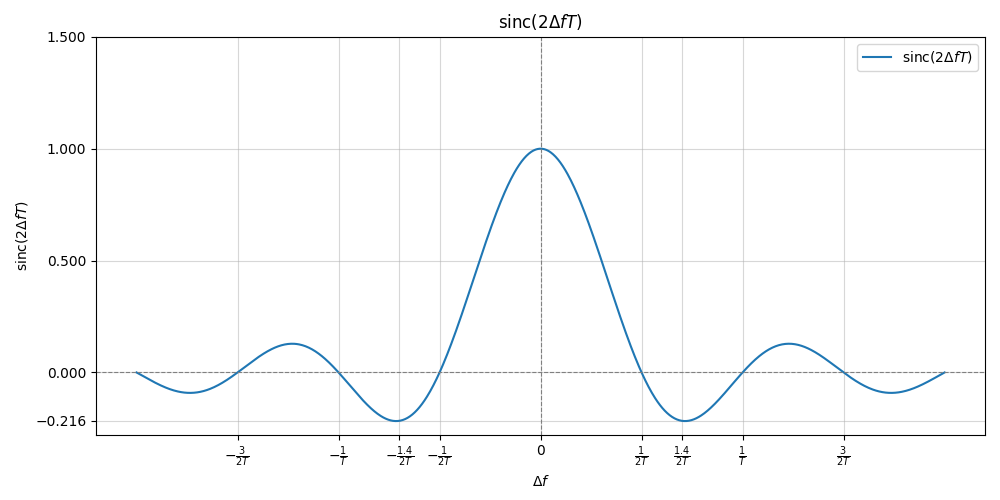
\includegraphics[width=0.5\textwidth]{sinc_plot.png}
            \caption{Plot of $\rho \approx \text{sinc}(2\Delta f T)$}
            \label{fig:sinc_plot}
        \end{figure}
    \end{enumerate}

    \item The minimum value in which $s_1(t)$ and $s_2(t)$ can be by setting the correlation coefficient to 0:
    \begin{align*}
        \rho &\approx \text{sinc}(2\Delta f T) = 0 \\
        \implies \Delta f &= \frac{1}{2T} \\
    \end{align*}

    \item We can find the probability of error by first finding the distance between the two signals:
    \begin{align*}
        d_{12}^2 &= \|s_2(t) - s_1(t)\|^2 \\
        &= \int_{-\infty}^{\infty} \left(s_2(t) - s_1(t)\right)^2 \, dt \\
        &= \int_{0}^{T} s_1^2(t) \, + dt \int_{0}^{T} s_2^2(t) \, dt -  \int_{0}^{T} 2s_1(t)s_2(t) \, dt \\
        &= \mathcal{E}_1 + \mathcal{E}_2 - 2\int_{0}^{T} s_1(t)s_2(t) \, dt \\
    \end{align*}

    Rearranging the equation for the correlation coefficient:
    \begin{align*}
        \sqrt{\mathcal{E}_1 \mathcal{E}_2} \rho = \mathcal{E}_b\rho &= \int_{-\infty}^{\infty} s_1(t)s_2(t) \, dt \\
    \end{align*}

    We can now use this relationship:
    \begin{align*}
        d_{12}^2 &= \mathcal{E}_1 + \mathcal{E}_2 - 2\mathcal{E}_b\rho \\
        &= 2\mathcal{E}_b - 2\mathcal{E}_b\rho \\
        d_{12} &= \sqrt{2\mathcal{E}_b(1 - \rho)} \\
    \end{align*}

    We can now find the probability of error given that the power spectral density of the noise is $\frac{N_0}{2}$:
    \begin{align*}
        P_e(\rho) &= Q\left(\frac{d_{12}}{\sqrt{2N_0}}\right) \\
        &= Q\left(\sqrt{\frac{\mathcal{E}_b(1 - \rho)}{N_0}}\right) \\
    \end{align*}        

    \item Since the $Q$ function is a monotonic decreasing function, we can find the minimum value of $P_e$ by finding the minimum value of $\rho$. This is because the minimum value of $\rho$ will give us the maximum input for the $Q$ function and will equate to the minimum value of $P_e$.
    
    We found that the minimum value of $\rho$ is:
    \begin{align*}
        \rho &= \text{sinc}(2\Delta f T) = 0 \\
        \implies \Delta f &= \frac{1}{2T} \\
        \implies P_e &= Q\left(\sqrt{\frac{\mathcal{E}_b}{N_0}}\right) \\
    \end{align*}

    Picking $\Delta f$ to be $\frac{1}{2T}$ will give us the minimum value of $P_e$.

    \item With this choice of $\Delta f$, the SNR needed to achieve the same probability of error as the case for binary antipodal is:
    \begin{align*}
        P_{e, \text{binary antipodal}} &= Q\left(\sqrt{\frac{2\mathcal{E}_b}{N_0}}\right) = Q\left(\sqrt{\text{SNR}}\right) \\
        P_{e, \text{binary FSK}} &= Q\left(\sqrt{\frac{\mathcal{E}_b}{N_0}}\right) = Q\left(\sqrt{\frac{1}{2}\text{SNR}}\right) \\
    \end{align*}

    Thus, we need double the SNR to achieve the same probability of error as the binary antipodal case. This gives us a 3 dB difference. Meaning, if we double the energy per bit, we can achieve the same probability of error as the binary antipodal case.

\end{enumerate}


% --------------------------------------------------------------------------------
% END BODY
% --------------------------------------------------------------------------------

\end{document}
